\chapter{Теоретические сведения.}

\section{Байесовский подход.}

\subsection{Основы байесовской статистики.}

Перед тем, как приступить к сетям, вспомним основы байесовской статистики.

Байесовская статистика противопоставляется частотной статистике, как альтернатива. Основное отличие в двух подходах состоит в том,
 что в байесовской статистике вероятность интерпретируется, как степень уверенности в истинности суждения. Другими словами, как мера незнания или неопределённости.
 В частотной статистике вероятность определяется как частота события. Байесовскую вероятность ещё иногда называют <<логической>> вероятностью, поскольку
 её проще применять в реальных задачах.

Байесовский подход же к оценке параметров заключается в утверждении, что априрорные знания влияют на апостериорные знания. Данное утверждение наиболее ярко видно в формуле Байеса:
$$P(H | D) = \frac{P(D | H)P(H)}{P(D)} = \frac{P(D | H)P(H)}{\int_{\mathcal{H}} P(D | \widetilde{H})P(\widetilde{H}) d\widetilde{H}}$$
$$P(H | D) \propto P(D | H)P(H)$$

В данной формуле,

$H$~---~некоторая гипотеза, вероятность которой мы хотим узнать, при помощи известных данных $D$.

$P(H | D)$~---~апостериорная вероятность гипотезы после того, как мы пронаблюдали данные $D$.

$P(H)$~---~это априорная вероятность или априорные знания о нашей гипотезе, которые мы знаем до того, как пронаблюдали данные $D$.

$P(D | H)$~---~плотность распределения, которое называется правдоподобием наблюдаемых данных $D$, если гипотеза верна.

$P(D)$~---~можно проинтерпретировать, как шум в данных. Особенно хорошо это заметно, когда мы записываем его в интегральной форме, где, как-бы, перебираем
 возможную гипотезу $\widetilde{H}$, которая должна наилучшим образом объяснить наши данные.

Нижняя запись, опуская знаменатель, который не зависит от $H$, обозначает пропорциональную зависимость между апостериорной вероятностью и априорной вероятностью.

Байесовские статические методы использует Теорему Байеса для вычисления и обновления вероятности после получения новых данных.

\subsection{Байесовский подход к оценке параметров.}

Теперь перейдем к задаче оценке параметров статистических(вероятностных) моделей. К таким моделям можно отнести почти все модели машинного обучения, нейронные сети, марковские цепи и др.

В общем случае обозначим за $a_{\theta}(x)$~---~статистическую модель из параметризованного семейства $\{a_{\theta}(x) : \theta \in \Theta\}$, где $\theta$~---~параметры модели. В случае
 линейной регрессии $y = w^T x + b$, $\theta = \{w, b\}$; для нейронных сетей $\theta$~---~веса промежуточных слоёв; для марковских цепях $\theta$ --- вероятности на рёбрах и т.д.

Когда мы занимаемся выбором модели $a_{\theta}(x)$, которая наилучшим образом(в некоторым смысле) описывают неизвестную закономерость в данных, то мы занимаемся подбором параметров $\theta$.
 В классическом подходе мы хотим найти \textit{точечную оценку} на параметры $\theta$, то есть найти значения параметров $\widehat{\theta}$, при котором качество нашей статистической модели будет наилучшим,
 т.е. $\widehat{\theta} = \displaystyle \argmin_{\theta} loss_{D_y, D_x}(\theta)$.
 Тут важно отметить, что нас интересует единственное такое оптимальное значение, даже если их может быть несколько. В этом и заключается точечный подход к оценке параметров.

Однако такой подход ничего не говорит про устойчивость найденного решения или, на языке байесовской статистики, уровня уверенности в том, что найденные $\widehat{\theta}$ является наилучшими.
 Чтобы лучше понять, рассмотрим пример с линейной регрессией $y = w^T x + b$ на двух ситуациях(Рисунок~\ref{fig:lin_reg1}, Рисунок~\ref{fig:lin_reg2}).

\begin{figure}[H]
    \begin{minipage}{0.48\textwidth}
        \centering
        \includegraphics[width=0.7\linewidth]{lin_reg1.png}
        \caption{Уверенная модель}
        \label{fig:lin_reg1}
    \end{minipage}
    \hfill
    \begin{minipage}{0.48\textwidth}
        \centering
        \includegraphics[width=0.7\linewidth]{lin_reg2.png}
        \caption{Неуверенная модель}
        \label{fig:lin_reg2}
    \end{minipage}
\end{figure}

И в первом, и во втором случае мы нашли оптимальную оценки $\widehat{w}, \widehat{b}$, однако во втором случае в данных сильно больше шума, что увеличвает
 неуверенность модели в том, что найденные оценки является наилучшими. Для того, чтобы лучше понимать ситуацию рассмотрим распредление параметров, а не их значение.
 Например, для примеров выше распределения параметров могли быть следующими:

\begin{figure}[H]
    \begin{minipage}{0.5\textwidth}
        \centering
        \includegraphics[width=0.8\linewidth]{w_estimator1.png}
        \caption{Уверенная модель}
        \label{fig:w_estimator1}
    \end{minipage}
    \hfill
    \begin{minipage}{0.5\textwidth}
        \centering
        \includegraphics[width=0.8\linewidth]{w_estimator2.png}
        \caption{Неуверенная модель}
        \label{fig:w_estimator2}
    \end{minipage}
\end{figure}

Таким образом, одного лишь значения оценки параметров $\widehat{\theta}$ может быть недостаточно для того, чтобы правильно решить поставленную задачу.
 Гораздо больше информации даёт распределение параметров $p(\theta)$, поэтому в байесовском подходе \textbf{оценивается не сами параметры, а их распределение.}

Далее мы применим основную байесовскую парадигму и добавим априорные знания в нашу статическую модель. Вернёмся к точечной оценке параметров:

$\widehat{\theta} = \displaystyle \argmin_{\theta} loss_{D_y, D_x} (\theta)$

Чаще всего в качество $loss_{D_y, D_x}(\cdot)$ предполагается брать $-\log p(D_y | D_x, \theta)$ и получаем:

$$\widehat{\theta} = \displaystyle \argmin_{\theta} (-\log p(D_y | D_x, \theta)) = \displaystyle \argmax_{\theta} \log p(D_y | D_x, \theta)$$

Получившаяся оценка $\widehat{\theta}$ называется \textit{оценкой максимума правдоподобия}($MLE$).
 В данном случае $\theta$ рассматривается, как неизвестный, но неслучайный параметр.

Теперь будем рассматривать $\theta$, как случайный параметр. Тогда будем искать значение $\theta$, которое максимизирует апостериорное распределение $p(\theta | D_y, D_x)$(или его логарифм, что тоже самое):
$$\widehat{\theta} = \displaystyle \argmax_{\theta} (\log p(\theta | D_x, D_y)) = \displaystyle \argmax_{\theta} (\log p(D_y | \theta, D_x) p(D_x | \theta) p(\theta) - \log p(D_y, D_x))$$
$$\widehat{\theta} = \Bigl[p(D_x | \theta) = p(D_x), т.к.\ D_x \independent \theta  \Bigr] = \displaystyle \argmax_{\theta} (\log p(D_y | \theta, D_x) p(D_x) p(\theta))$$
$$\widehat{\theta} = \displaystyle \argmax_{\theta} (\underbrace{\log p(D_y | \theta, D_x)}_{-\mathcal{L}_{D_y, D_x}(\theta)}+ \underbrace{\log p(\theta)}_{-\mathcal{R}(\theta)})$$

Таким образом мы получили \textit{оценку апостериорного максимума}($MAP$) на параметры $\theta$. Стоит заметить, что разница между итоговым оптимизируемым функционалом в случае $MLE$ и случае $MAP$ заключется в добавлении функционала $\mathcal{R}(\theta)$,
 который выступает в роли \textit{регуляризатора} весов.

Таким образом добавление априорных знаний или априрорного распределения параметров также добавляет естественный регуляризатор в функционал. Следовательно, просто меняя подход на байесовский наша модель становится более устойчива к переобучению.

\textbf{Замечание.} В будущем мы ещё вернёмся к нашему оптимизируемому функционалу, добавляя в него дополнительные слагаемые и тем самым получая новые свойства.
 Здесь также можно проследить интересный переход от вероятностной постановки задачи к оптимизационной, которую мы решаем с помощью градиентных методов.

\section{Вариационный вывод.}

Теперь попробуем совместить все предыдущие идеи в одну. Такое решение было предложено в \cite{hoffman-SVI}.

Рассмотрим вероятностную модель $p(\underbrace{D_x, D_y}_{\mathcal{D}}, \theta) = p(\theta | D_x, D_y) p(D_x, D_y)$, где $D_x = (x_1, x_2, ..., x_n)$,
 $D_y = (y_1, y_2, ..., y_n)$, $n \gg 1$, $\theta \in \mathbb{R}^d$

Для получения апостериорного распределения на параметры $\theta$ воспользуемся формулой Байеса:

$$p(\theta | D_x, D_y) = \frac{p(D_x, D_y | \theta) p(\theta)}{p(D_x, D_y)} = \frac{p(D_y) | \theta, D_x) p(\theta)}{p(D_x, D_y)} + const$$
$$p(\theta | D_x, D_y) = \frac{\sum_{i=1}^n p(y_i | \theta, x_i) p(\theta)}{\int p(D_x, D_y | \widetilde{\theta})p(\widetilde{\theta}) d\widetilde{\theta}} + const$$

Подсчёт истинного апостериора таким способом требует взятие интеграла в знаменателе. В случаях, когда это возможно, проблем нет. Однако в большинстве случаев, которые используются на практике и которые нас интересуют, такой интеграл не берётся.

\subsection{KL-дивергенция и вариационная нижняя оценка.}

Для решения проблемы будем пробовать приблизить апостериорное распределение $p(\theta | D_x, D_y)$ параметризованным распределением $q(\theta | \varphi)$ путём минимизации дивергенции Кульбака-Лейблера $KL(q(\theta | \varphi)\ ||\ p(\theta | D_x, D_y))$.
 То есть
$$\widehat{\varphi} = \argmin_{\varphi} KL(q(\theta | \varphi)\ ||\ p(\theta | D_x, D_y))$$
Чем плоха такая оптимизационная задача? Для того, чтобы считать значение самой функции и её градиента, нам бы потребовалось уметь считать значение $p(\theta | D_x, D_y)$, которое мы и пытаемся найти. Если бы могли его считать, то
 и смысла в нашей задаче не было бы. Поэтому требуется найти альтернативный оптимизируемый функционал.

Распишем дивергенцию:
$$KL(q(\theta | \varphi)\ ||\ p(\theta | D_x, D_y))) = \int q(\theta | \phi) \log \frac{q(\theta | \varphi)}{p(\theta | D_x, D_y)} d\theta = \int q(\theta | \varphi) \log q(\theta | \varphi)-$$
$$-\int q(\theta | \varphi) \log p(\theta | D_x, D_y) = \mathbb{E}_{\theta \sim q(\theta | \varphi)} [\log q(\theta | \varphi)] - \mathbb{E}_{\theta \sim p(\theta | D_x, D_y)}[\log p(\theta | D_x, D_y)]=$$
$$=\underbrace{\mathbb{E}_{\theta \sim q(\theta | \varphi)} [\log q(\theta | \varphi)] - \mathbb{E}_{\theta \sim p(\theta | D_x, D_y)}[\log p(\theta, D_x, D_y)] }_{-ELBO(\varphi, \mathcal{D})} + \underbrace{\log p(D_x, D_y)}_{const}$$

Тогда получаем следующее:
$$KL(q(\theta | \varphi)\ ||\ p(\theta | D_x, D_y)) + ELBO(\varphi, \mathcal{D}) = \log p(D_x, D_y)$$

Получившееся значение $ELBO(\varphi, \mathcal{D})$ называется \textit{вариационной нижней оценкой} или \textit{evidence lower bound}. Оно также записывается,
 как $L(\varphi, \mathcal{D})$.

Свойства вариационной нижней оценки:
\begin{itemize}
    \item $\log p(D_x, D_y) \ge L(\varphi, \mathcal{D}) = \mathbb{E}_{\theta \sim q(\theta | \varphi)} [\frac{\log p(\theta, D_x, D_y)}{q(\theta | \varphi)}]$, т.к. дивергенция Кульбака-Лейблера неотрицательна. Данное неравенство верно для любого распределения $q$.
    \item $L(\varphi, \mathcal{D}) \le 0$, т.к. $\log p(D_x, D_y) \le 0$. Т.е. вариационная нижняя оценка всегда неположительна.
\end{itemize}

Следовательно, задача о минимизации дивергенции Кульбака-Лейблера по параметрам $\varphi$ эквивалентна задаче о максимизации вариационной нижней оценки по тем же параметрам $\varphi$. Этим
 фактом мы можем пользоваться, чтобы перейти от предыдущей оптимизационной задаче, которая требовала подсчёта апостериорной вероятности $p(\theta\ |\ D_x, D_y)$, к
 задаче, где этого не требуется. Тем самым это упрощает нашу оптимизационную задачу:
$$\widehat{\varphi} = \argmin_{\varphi} KL(q(\theta | \varphi)\ ||\ p(\theta | D_x, D_y)) = \argmax_{\varphi} L(\varphi, \mathcal{D})$$
$$\widehat{\varphi} = \argmin_{\varphi} -L(\varphi, \mathcal{D})$$
Распишем $-L(\varphi, \mathcal{D})$:
$$-L(\varphi, \mathcal{D}) =  \mathbb{E}_{\theta \sim q(\theta | \varphi)} [\log q(\theta | \varphi)] -
\mathbb{E}_{\theta \sim q(\theta | \varphi)} [\log p(D_y | \theta, D_x)] - \mathbb{E}_{\theta \sim q(\theta | \varphi)} [p(\theta)] - \log p(D_x)$$
Теперь попробуем провести аналогию между оптимизационной задачей в предыдущем пункте и новой. Это будет лишь приблизительная аналогия с теоретической точки зрения,
 однако на практике её всегда можно считать истинной:
$$\underbrace{\mathbb{E}_{\theta \sim q(\theta | \varphi)} [\log q(\theta | \varphi)]}_{-\mathcal{H}(\varphi)} -
\underbrace{\mathbb{E}_{\theta \sim q(\theta | \varphi)} [\log p(D_y | \theta, D_x)]}_{-\mathcal{L}_{D_x,D_y}(\varphi)} -
\underbrace{\mathbb{E}_{\theta \sim q(\theta | \varphi)} [\log p(\theta)]}_{-\mathcal{R}(\varphi)} - \underbrace{\log p(D_x)}_{-noise}$$

Тогда наша функция потерь переписывается в виде:
$$-L(\varphi, \mathcal{D}) = \mathcal{L}_{D_x,D_y}(\varphi) + \mathcal{R}(\varphi) + noise - \mathcal{H}(\varphi),$$
где

$\mathcal{L}_{D_x,D_y}(\varphi)$ --- функция ошибки предсказания модели.

$\mathcal{R}(\varphi)$ --- естественный регуляризатор, получившийся от передачи априорных знаний в модель.

$\mathcal{H}(\varphi)$ --- энтропия Шеннона параметрического распределения $q(\theta | \varphi)$. Чем выше этот параметр, тем более "хаотичным" можно считать
 получившееся распредление. Вместе с тем уровень энтропии показывает уровень уверенности в значение параметров нашей модели. Например, значение энтропии Шеннона
 $\delta$-распределения равно 0.

$noise$ --- шум в данных, от которого нам не избавиться, но он является константой, поэтому из оптимизируемого функционала его можно исключить.

\subsection{Стохастический вариационный вывод.}

Для решения оптимизационной задачи можно использовать различные методы: методы 1-го порядка(градиентные методы), методы второго порядка(метод Ньютона), генетические и эволюционные алгоритмы. Поскольку мы работаем с большими объёмами данных,
 как по количеству самих данных, так и по количеству признаков, то самыми эффективными будут градиентные методы.

Тогда посчитаем градиент по $\varphi$:
$$\nabla_{\varphi} (-L(\varphi, \mathcal{D})) = \nabla_{\varphi} \mathcal{L}_{D_x, D_y}(\varphi) + \nabla_{\varphi} \mathcal{R}(\varphi) - \nabla_{\varphi} \mathcal{H}(\varphi)=$$
$$= -\nabla_{\varphi} \mathbb{E}_{q(\theta | \varphi)}[\log p(D_y | \theta, D_x)] - \nabla_{\varphi} \mathbb{E}_{q(\theta | \varphi)} [\log p(\theta)] +
\nabla_{\varphi} \mathbb{E}_{q(\theta | \varphi)} [\log q(\theta | \varphi)]$$
% $$= -\mathbb{E}_{ q(\theta | \varphi)}[\nabla_{\varphi}\log p(D_y | \theta, D_x)] - \mathbb{E}_{q(\theta | \varphi)} [\nabla_{\varphi} \log p(\theta)] +
% \mathbb{E}_{q(\theta | \varphi)} [\nabla_{\varphi} \log q(\theta | \varphi)]$$

Вернёмся к интегральной форме:
$$-\nabla_{\varphi} \int q(\theta | \varphi) \log p(D_y | \theta, D_x) d\theta - \nabla_{\varphi} \int q(\theta | \varphi) \log p(\theta) d\theta + \nabla_{\varphi} \int q(\theta | \varphi) \log q(\theta | \varphi) d\theta$$

Нам было бы удобно, если бы функция плотности $q(\theta | \varphi)$ не зависила от параметров, поскольку тогда мы могли бы поднести знак дифференцирования под символ матожидания. Однако пока что мы так делать не можем.

Вместо этого попробуем внести дифференцирование под знак интеграла. Это возможно при соблюдении определённых \textit{условий регулярности}, которые мы накладываем на статистическую модель. Такие модели также называются
 \textit{регулярными}\cite{medvedev-stats}. Сначал рассмотрим последний интграл:
$$\int \frac{\partial}{\partial\varphi} (q(\theta | \varphi) \log q(\theta | \varphi)) d\theta = \int \frac{\partial}{\partial\varphi} q(\theta | \varphi) \log q(\theta | \varphi) d\theta\ +\ \int q(\theta | \varphi) \frac{\partial}{\partial\varphi} \log q(\theta | \varphi) d\theta =$$
$$=\int \frac{\partial}{\partial\varphi} q(\theta | \varphi) \log q(\theta | \varphi) d\theta\ +\ \int \frac{\partial}{\partial\varphi} q(\theta | \varphi) d\theta = \int \frac{\partial}{\partial\varphi} q(\theta | \varphi) \log q(\theta | \varphi) d\theta = $$
$$=\int q(\theta | \varphi) \frac{1}{q(\theta | \varphi)} \frac{\partial}{\partial\varphi} q(\theta | \varphi) \log q(\theta | \varphi) d\theta = \int q(\theta | \varphi) \frac{\partial(\log q(\theta | \varphi))}{\partial\varphi} \log q(\theta | \varphi) d\theta=$$
$$=\mathbb{E}_{\theta \sim q(\theta | \varphi)} \Bigl[\frac{\partial(\log q(\theta | \varphi))}{\partial\varphi} \log q(\theta | \varphi)\Bigr]$$

Таким образом мы смогли занести $\frac{\partial}{\partial\varphi}$ под матожидание. В последних переходах использовался \textit{log-derivative trick}, который позволяет перейти к производной от логарифма плотности, оставив при этом, матожидание.
 Аналогично поступим для двух остальных интегралов:
$$-\int \frac{\partial}{\partial\varphi} q(\theta | \varphi) (\log p(D_y | \varphi, D_x) + \log p(\theta)) d\theta =$$
$$=-\int q(\theta | \varphi) \frac{\partial (\log q(\theta | \varphi))}{\partial\varphi} (\log p(D_y | \theta, D_x) + \log p(\theta)) d\theta$$
Тогда итоговый градиент функции потерь будет равен:
$$\frac{\partial}{\partial\varphi} (-L(\varphi, \mathcal{D})) = \int q(\theta | \varphi) \frac{\partial \log q(\theta | \varphi)}{\partial\varphi} (\log q(\theta | \varphi) - \log p(D_y | \theta, D_x) - \log p(\theta)) d\theta$$
Этот интеграл мы не можем посчитать аналитически, поэтому воспользуемся методом Монте-Карло для получения приближенной оценки интеграла\cite{black-box-vi}:
$$\theta_k \sim q(\theta | \varphi),\ k = \overline{1...K}$$
$$\grad (-L(\varphi, \mathcal{D})) \approx \displaystyle \frac{1}{K}\sum_{k=1}^{K} \frac{\partial(\log q(\theta_k | \varphi))}{\partial\varphi} (\log q(\theta_k | \varphi) - \log p(D_y | \theta_k, D_x) - \log p(\theta_k))$$
Однако на практике время сэмплирования $\theta_k$ занимает достаточно много времени, поэтому часто берут $K=1$. Для больших данных мы часто пользуются стохастическим градиентом:
$$j \sim U[1...N]$$
$$\theta_k \sim q(\theta | \varphi),\ k = \overline{1...K}$$
$$\grad (-L(\varphi)) \approx \displaystyle \frac{1}{K}\sum_{k=1}^K \frac{\partial(\log q(\theta_k | \varphi))}{\partial\varphi} (\log q(\theta_k | \varphi) - N\log p(y_j | \theta_k, x_j) - \log p(\theta_k))$$
Также для нейронных сетей используется пакетный градиентный спуск, чтобы мы могли обрабатывать данные небольшими пакетами. Такой подход уменьшает дисперсию:
$$i_b \sim U[1...N],\ b = \overline{1...B}$$
$$\theta_k \sim q(\theta | \varphi),\ k = \overline{1...K}$$
$$-\frac{dL}{\partial\varphi}\approx\frac{1}{K} \sum_{k=1}^K \Bigl[\frac{\partial(\log q(\theta_k | \varphi))}{\partial\varphi} \bigl(\log q(\theta_k | \varphi) - \frac{N}{B} \sum_{b=1}^B (\log p(y_{i_b} | \theta_k, x_{i_b})) - \log p(\theta_k)\bigr)\Bigr]$$

Однако данный метод перестаёт работать при $N \gg 1$ и $|\varphi| \gg 1$ из-за очень большой дисперсии градиента.
 Поскольку $\mathbb{E}_{\theta \sim q(\theta | \varphi)} \Bigl[\frac{\partial(\log q(\theta | \varphi))}{\partial \varphi}\Bigr] = 0$,
 то в после сэмплирования $\theta_k$ мы будем получать числа разных знаков. При этом второй множитель из-за домножения на $\frac{N}{B}$
 будет очень большим по норме, и из-за этого дисперсия будет очень большого порядка с постоянно меняющимся знаком.

 Из-за этого при больших данных данный метод неприменим и нужно искать ему замену. Оригинально данный алгоритм был назван REINFORCE и был придуман
 в обучении с подкреплением \cite{williams:92}.

\subsection{Трюк с репараметризацией.}

На замену этому методу был придуман метод, который называется \textit{трюк с репараметризацией} (\textit{reparametrization trick})\cite{auto-encod-bayes}.
 Предварительно запишем несколько утверждений утверждений:

\begin{proposition}
    (Law of the unconscious statistician)
    \label{LOTUS}
    Пусть $z$ - случайный вектор, $z \sim p(z)$. При этом существует случайный вектор $\varepsilon \sim r(\varepsilon)$ и существует диффеоморфизм $g$: $z = g(\varepsilon)$ такой,
     что $g(\varepsilon) \sim p(z)$. Тогда
    $$\forall f -\ измеримая\ функция\ случ.\ величины$$
    $$\mathbb{E}_{p(z)}[f(z)] = \mathbb{E}_{r(\varepsilon)}[f(g(\varepsilon))]$$
    $$\int p(z) f(z) dz = \int r(\varepsilon) f(g(\varepsilon)) d\varepsilon$$
\end{proposition}

Таким образом данное утверждение позволяет заменять одну сэмплируемую величину на другую, сохраняя матожидание. Это свойство
 применимо для нашей предыдущей опимизационной задаче:
$$-L(\varphi) = \mathbb{E}_{q(\theta | \varphi)}[\log q(\theta | \varphi)] - \mathbb{E}_{q(\theta | \varphi)}[\log p(D_y | \theta, D_x)] - \mathbb{E}_{q(\theta | \varphi)}[\log p(\theta)]$$

Предположим, что мы можем некоторым способом репараметризовать нашу модель. То есть найти диффеоморфизм $g$: $\theta = g(\varepsilon, \varphi)$, $\varepsilon \sim r(\varepsilon)$.
 При этом $g(\varepsilon, \varphi) \sim q(\theta | \varphi)$. Тогда, используя \ref{LOTUS} мы можем переписать функцию потерь:
$$-L(\varphi) = \mathbb{E}_{r(\varepsilon)}[\log q(g(\varepsilon, \varphi) | \varphi)] - \mathbb{E}_{r(\varepsilon)}[\log p(D_y | g(\varepsilon, \varphi), D_x)] - \mathbb{E}_{r(\varepsilon)}[\log p(g(\varepsilon, \varphi))]$$
В полученной формуле мы добились того, чего хотели раньше --- плотность больше не зависит от оптимизируемых параметров $\varphi$, и следовательно мы можем занести производную под символ матожидания без ошибки:
$$\frac{\partial}{\partial\varphi} \mathbb{E}_{r(\varepsilon)}[\log q(g(\varepsilon, \varphi) | \varphi)] -
\frac{\partial}{\partial\varphi}\mathbb{E}_{r(\varepsilon)}[\log p(D_y | g(\varepsilon, \varphi), D_x)] -
\frac{\partial}{\partial\varphi} \mathbb{E}_{r}[\log p(g(\varepsilon, \varphi))]=$$
$$=\mathbb{E}_{r(\varepsilon)}\bigl[\frac{\partial}{\partial\varphi} \log q(g(\varepsilon, \varphi) | \varphi)\bigr] -
\mathbb{E}_{r(\varepsilon)}\bigl[\frac{\partial}{\partial \varphi} \log p(D_y | g(\varepsilon, \varphi), D_x)\bigr] -
\mathbb{E}_{r(\varepsilon)}\bigl[\frac{\partial}{\partial\varphi} \log p(g(\varepsilon, \varphi))\bigr]$$
Теперь для получения приближения градиента мы используем метод Монте-Карло для оценки матожиданий:
$$\varepsilon_k \sim r(\varepsilon),\ k=\overline{1...K}$$
$$\theta_k = g(\varepsilon_k, \varphi)$$
$$\frac{\partial (-L(\varphi))}{\partial\varphi} \approx \frac{1}{K} \sum_{k=1}^K \frac{\partial}{\partial\varphi} \log q(\theta_k | \varphi) -
\frac{\partial}{\partial\varphi} \log p(D_y | \theta_k, D_x) -
\frac{\partial}{\partial\varphi} \log p(\theta_k)$$
Аналогично мы можем написать стохастическую оценку на градиент:
$$\varepsilon_k \sim r(\varepsilon),\ k=\overline{1...K}$$
$$\theta_k = g(\varepsilon_k, \varphi)$$
$$j \sim U[1...N]$$
$$\frac{\partial (-L(\varphi))}{\partial\varphi} \approx \frac{1}{K} \sum_{k=1}^K \frac{\partial}{\partial\varphi} \log q(\theta_k | \varphi) -
N\frac{\partial}{\partial\varphi} \log p(y_j | \theta_k, x_j) -
\frac{\partial}{\partial\varphi} \log p(\theta_k)$$
И пакетный градиент, который чаще используется при обучении моделей для работы с большими данными:
$$\varepsilon_k \sim r(\varepsilon),\ k=\overline{1...K}$$
$$\theta_k = g(\varepsilon_k, \varphi)$$
$$i_b \sim U[1...N],\ b=\overline{1...B}$$
$$\frac{\partial (-L(\varphi))}{\partial\varphi} \approx \frac{1}{K} \sum_{k=1}^K \Bigl(\frac{\partial}{\partial\varphi} \log q(\theta_k | \varphi) -
\frac{N}{B}\sum_{b=1}^B \frac{\partial}{\partial\varphi} \log p(y_{i_b} | \theta_k, x_{i_b}) -
\frac{\partial}{\partial\varphi} \log p(\theta_k)\Bigr)$$

\chapter{Виды нейронных сетей.}

\section{Детерминированные нейронные сети.}

Сначала напомним, что такое обычные(детерминированные) нейронные сети и как они обучаются.

Основная задача обычных искусственных нейронных сетей($ANN$) в том, чтобы аппроксимировать некоторую зависимость выхода $y$ от
 входа $x$: $y = \Phi(x)$. Зависимость $\Phi(x)$ аппроксимируем через композицию последовательных преобразований.

Для простоты будем рассматривать обычные \textit{полносвязные} сети со входом $x$,
 скрытыми(промежуточными) состояниями слоёв $\bm{h_i}$, функциями активации $a_i(\cdot)$ и выходом $y$:
$$\bm{h_0} = \bm{x}$$
$$\bm{h_i} = a_i(\bm{W_i} \cdot h_{i-1} + \bm{b_i}), i = \overline{1...n}$$
$$\bm{h_n} = \widehat{y}$$
$$L = \mathcal{L}(\widehat{y}, y),$$ где $\mathcal{L}(\cdot, \cdot)$ - функция ошибки.

Обозначим параметры модели на $i$-ом слое $\bm{\theta_i} = (\bm{W_i}, \bm{b_i})$, а параметры всей модели через $\bm{\Theta} = \{\bm{\theta_i} :~i~=~\overline{1...n}\}$.
Чаще всего нейронные сети принято рассматривать, как вычислительный граф/граф вычислений.
 Такой подход удобен с инженерной точки зрения, поскольку позволяет воспользоваться инструментом автоматического
 дифференцирования, и используется во всех современных фреймоворках: PyTorch, TensorFlow и прочие.
 Граф вычислений является ациклическим ориентированным графом, составленным из вершин-переменных и вершин-операций(Рисунок~\ref{fig:ANN}).
\begin{figure}[H]
    \centering
    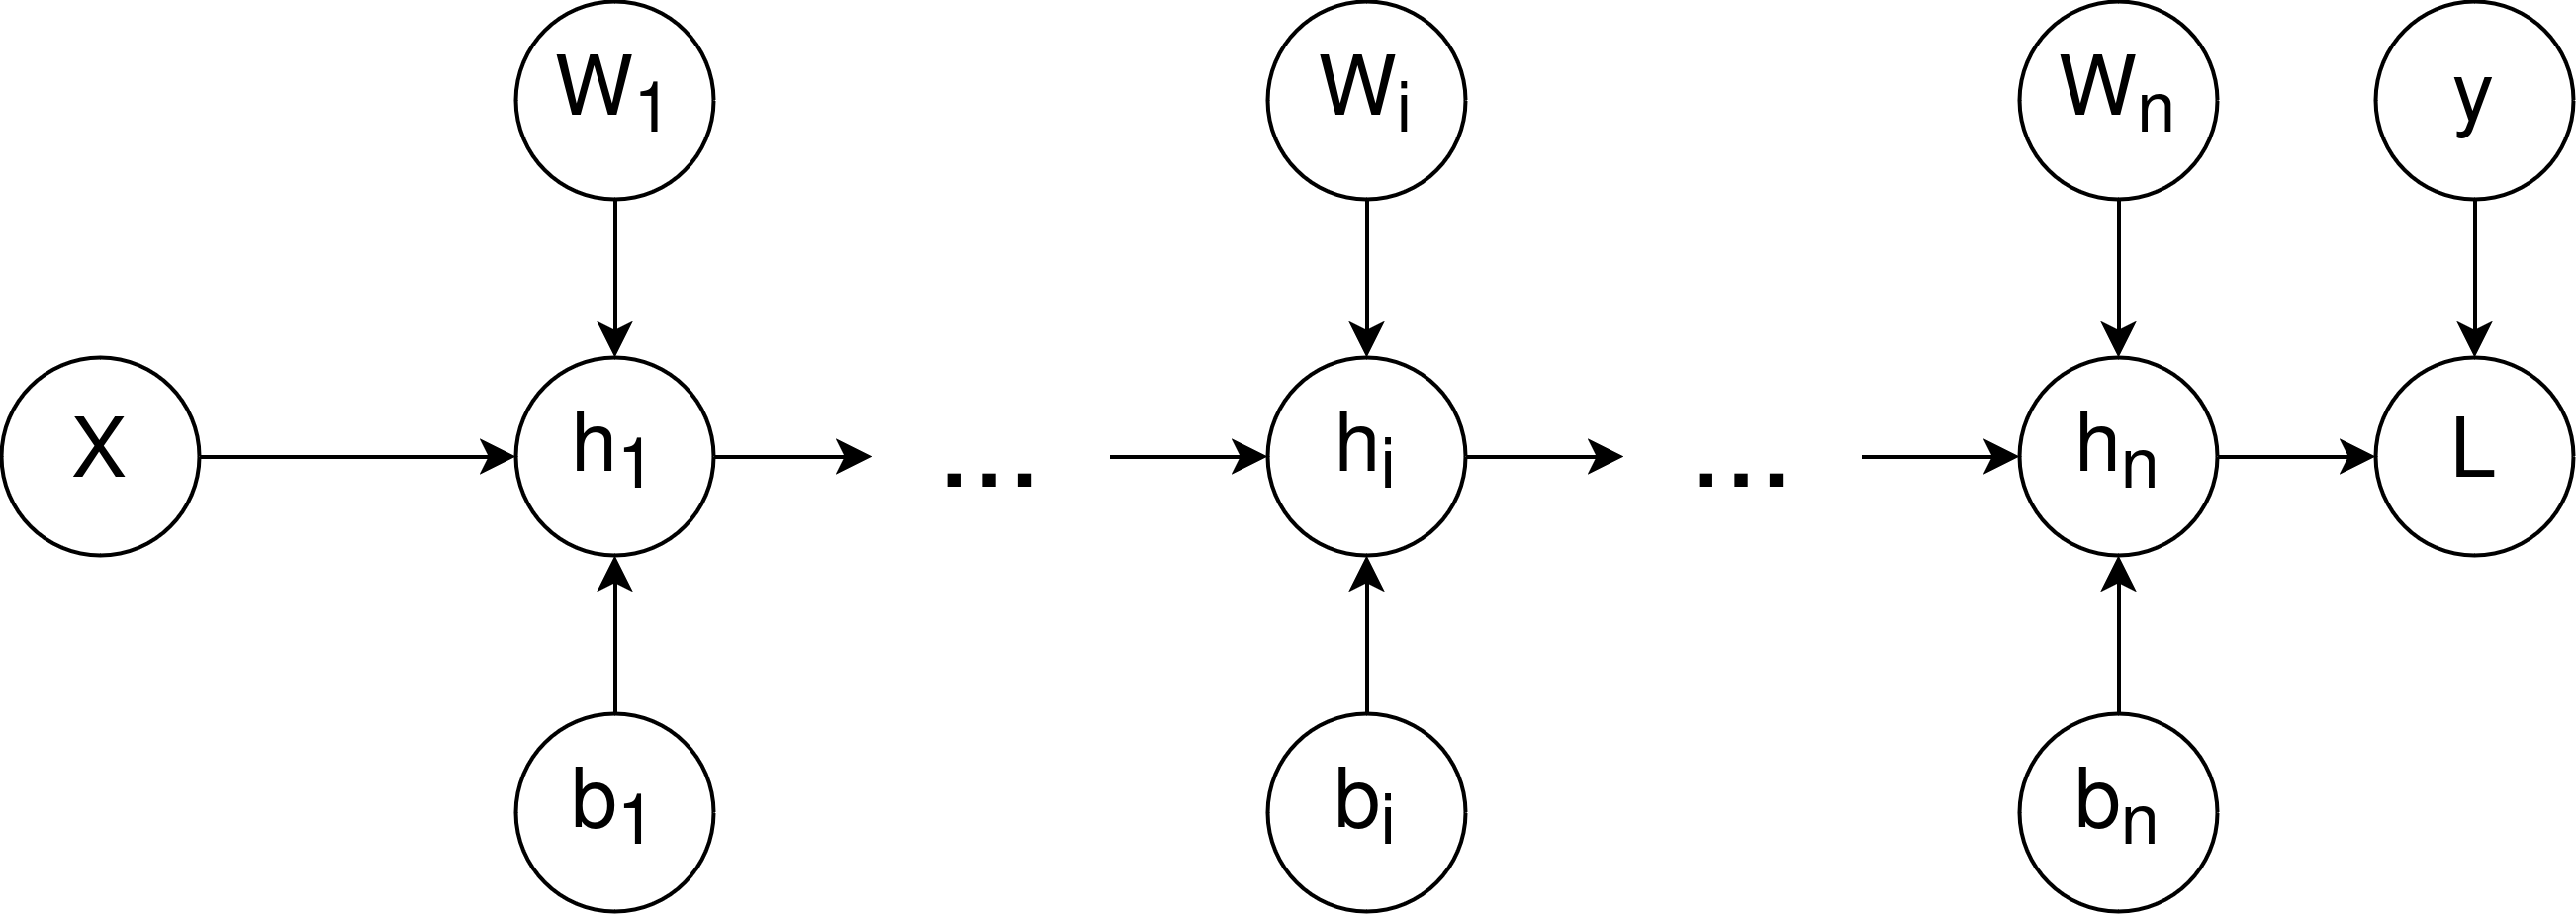
\includegraphics[width=0.7\linewidth]{ANN.png}
    \caption{\textit{Полносвязная} сеть в виде графа вычислений}
    \label{fig:ANN}
\end{figure}

Далее будем называть модели, основанные на графах вычислений, --- графовыми моделями. Графы вычислений могут разных типов:
 статическими/динамическими, детерминированными/вероятностными и т.д. Для обучения/настройки параметров детерминированных графовых моделей
 используется метод \textit{обратного распространения ошибки(back propagation)}, который широко используется в современном мире. Вкратце напомним алгоритм:

После прямого выполнения графа(\textit{forward pass}), то есть в соответствии с направлениями рёбер на выходе мы получаем
 $L$ -значение функции ошибки, которые в зависимости от задач мы хотим либо минимизировать, либо максимизировать. Для этого
 мы пользуемся градиентными методами оптимизации, что требует вычисление градиентов $\frac{dL}{d W_i}, \frac{dL}{d b_i}$ по нашим параметрам модели, где $i = \overline{1,n}$.
 В общем случае это трудная задача, однако в случае детерминированных графовых моделей мы можем использовать цепное правило(\textit{chain rule}) для того, чтобы последовательно
 проталкивать градиенты, начиная с концевой вершины, содержащей $L$.

 Например, для подсчёта градиентов $\frac{dL}{d W_n}, \frac{dL}{d b_n}$ мы представим его в виде
 $$\frac{dL}{d W_n} = \frac{dL}{d h_n} \cdot \frac{d h_n}{d W_n}$$
 $$\frac{dL}{d b_n} = \frac{dL}{d h_n} \cdot \frac{d h_n}{d b_n}$$

Аналогично для всех остальных параметров модели мы будем проталкивать накопленный с концевой вершины градиент до соответствующих вершин и
 с помощью этого градиента высчитывать градиент по параметрам модели. Схему работы алгоритма обратного распространения ошибки
 можно увидеть на Рисунок~\ref{fig:ANN_back_prop}.
\begin{figure}[H]
    \centering
    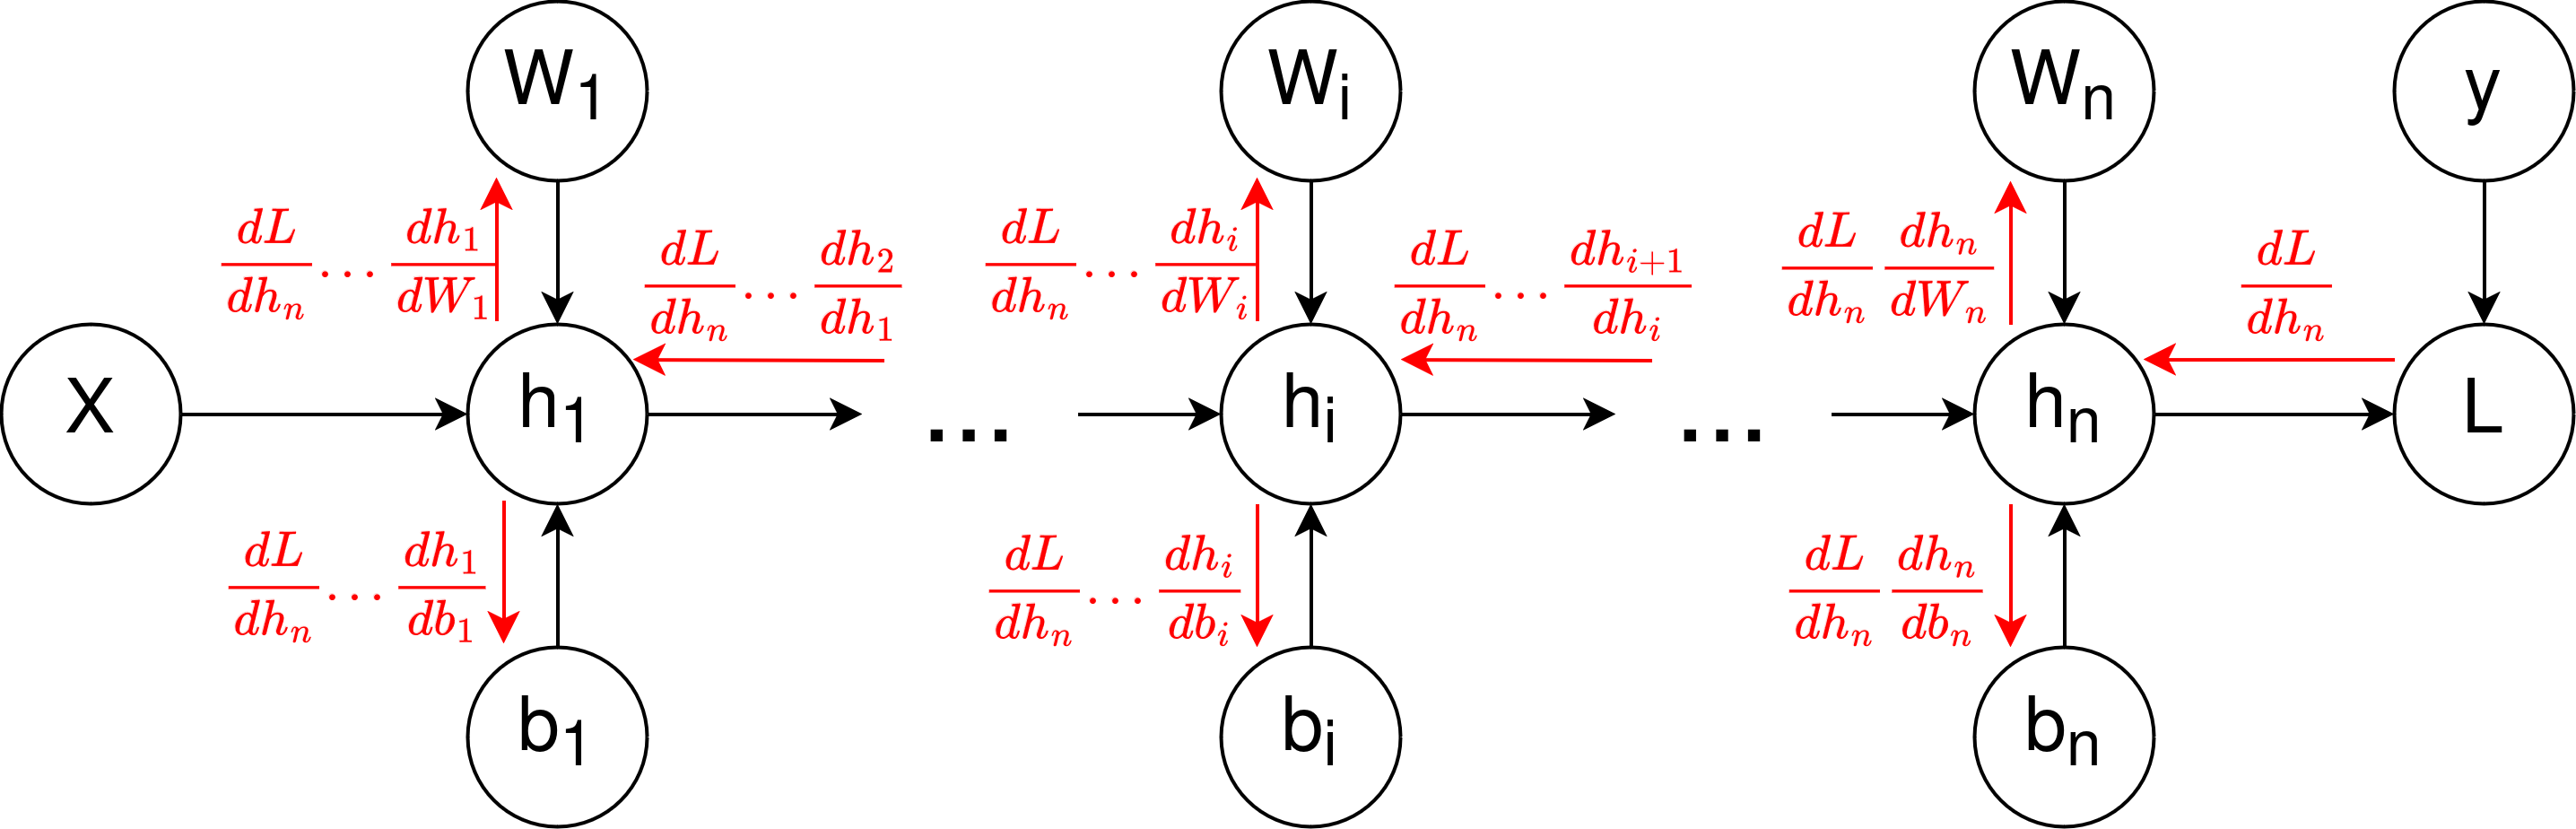
\includegraphics[width=0.7\linewidth]{ANN_back_prop.png}
    \caption{Обратное распространение ошибки по графу вычислений детерминированной полносвязной сети}
    \label{fig:ANN_back_prop}
\end{figure}

Однако детерминированные нейронные сети обладают несколькими проблемами:
\begin{itemize}
    \item Переобучение.
    \item Низкая интерпретируемость.
    \item Завышенная/заниженная уверенность модели в предсказаниях, даже если они неверные.
    \item Низкий уровень откалиброванности модели.
    \item Избыток параметров.
\end{itemize}

Указанные проблемы попытаемся решить с помощью байесовского подхода к нейронным сетям, который
 рассмотрим далее.

\section{Байесовские нейронные сети.}
\subsection{Вероятностные графы вычислений.}

Перед тем, как приступить к байесовским нейронным сетям, рассмотрим \textit{вероятностные графы вычислений}, на которых основаны
 байесовские сети. В литературе также часто вместо названия \textit{вероятностные графы вычислений} встречается \textit{вероятностные графические модели}.
 Второе название является более общим, в то время как первое более специфично именно для байесовских нейронных сетей.
 Такие графы вычислений широко используются и известны достаточно давно. Они лежат в основе, например,
 Марковских цепей, которые ранее активно использовались в различных задачах машинного предсказания, распознавания образов и т.п.

Основная мотивация в использовании вероятностного подхода состоит в том, что в реальном мире мы чаще имеем дело с неопределённостью в данных и знаниях
 и не можем детерминированно описать все приходящие переменные для решения задачи. Для решения проблем с неопределённостью
 можно попробовать собрать большие объёмы данных для того, чтобы попытаться "понять" эту неопределённость. С другой стороны
 мы можем использовать байесовский подход, который напрямую оперирует с неопределённостью.

Рассмотрим структуру \textit{вероятностных графовых моделей}. В отличие от детерминированных моделей в граф добавляются вершины
 со случайными переменными. Таким образом в нашем совместно существуют детерминированные вершины и случайные (Рисунок \ref{fig:PGM_example}). Стоит отметить,
 что после вступления в контакт детерминированных переменных и случайных, весь дальнейший результат будет случайным.
 При работе с такими моделями нужно различать \textit{наблюдаемые} и \textit{скрытые/латентные} переменные.
 Различия в этих двух понятиях естественны: в реальной жизни у нас есть некоторые известные данные и те, которые мы не может измерить явно,
 а лишь вычислить в результате работы модели.

\begin{figure}[H]
    \centering
    \includegraphics[width=0.7\linewidth]{PGM_example.png}
    \caption{Вероятностная графическая модель. Здесь круги с пунктирной границей являются сэмплируемыми случайными величинами. Зелёным цветом обозначены наблюдаемые случайные переменные.}
    \label{fig:PGM_example}
\end{figure}

Стоит сделать замечание, что детерминированные переменные также можно представить,
 как случайные величины с $\delta$-функцией плотности распределения $\delta(\cdot)$,
 где $\delta(\cdot)$ --- $\delta$-функция Дирака. Данный факт позволяет рассматривать все вершины
 в вероятностной графовой модели, как случайные.

Введём более строгое определение. Пусть $(x_1, x_2, ..., x_n)$ - множество случайных величин, представляющих вершины
 ориентированного графа. Тогда \textit{вероятностная графическая модель} --- это семейство условных распределений $p(x_1 | ...)$, $p(x_2 | ...)$ и т.д. над
 данными случайными величинами $x_1, x_2, x_3, ..., x_n$.

В случае графовых моделей каждая случайная величина $x_i$ зависит не от всех других случайных
 величин, а лишь от некоторого множество её предков $ancestors(x_i)$.
 Таким образом мы можем вычислить полную условную плотность величины $x_i$ так:
$$p(x_i | x_n, x_{n-1}, ... x_1) = p(x_i | ancestors(x_i))$$

Используя \textit{цепное правило} для совместного распределения $p(x_1, x_2, ..., x_n)$ мы можем расписать его
 через частные распределения и условные:
$$p(x_1, x_2, ..., x_n) = p(x_1) p(x_2 | x_1) p(x_3 | x_2, x_1) ... p(x_n | x_{n-1}, ..., x_1)$$

Выбирая порядок множителей справа удобным образом мы можем вычислить совместное распределение.

Подобные \textit{вероятностные графические модели} позволяют узнавать неочевидные взаимосвязи в данных, если в качестве
 вершин принять, например, признаки из какого-нибудь набора данных. При достаточном времени, потраченном на составлении связей в данном графе,
 аналитик данных способен в удобной форме отлавливать закономерности и проверять гипотезы о распределении данных. Также возможно их использование в
 системном или бизнес анализах, однако придётся потратить больше времени для дизайна нашего графа, поскольку мы можем столкнуться с не числовыми вершинами, а, например, событийными.

Другая полезная особенность таких моделей в том, что вместо какого-то конкретного значения интересующей нас величины мы получаем её распределение(Рисунок \ref{fig:PGM_pdf}).
 Это даёт сильно больше информации, чем одно значение и позволяет оценивать \textit{риски}, связанные с этой величиной. Существует много задач, где определение рисков важнее
 какого-то одного ответа. Примеры: задача кредитного скоринга, большинство задач по работе с финансами(определение стоимости ценных бумаг, курса валют и т.д.), задачи в области медицины
 и здравоохранения, транспорт на автопилоте и т.п.

\begin{figure}[H]
    \centering
    \includegraphics[width=0.7\linewidth]{PGM_pdf.png}
    \caption{Та же графическая модель, но с видимыми распределениями значений в вершинах. Детерминированные вершины имеют $\delta$-функцию распределения.}
    \label{fig:PGM_pdf}
\end{figure}

Существуют несколько инструментов для работы с такими моделями: Bayes Net Toolbox ($\verb|MATLAB|$), pgmpy ($\verb|Python|$) и др.

\subsection{Байесовские нейронные сети.}

Теперь рассмотрим байесовский подход к нейронным сетям. Такие сети в некоторой литературе называются -- \textit{байесовские нейронные сети}.

\textbf{Стоит отметить}, что байесовские сети/графы(bayes nets, bayes networks) и байесовские нейронные сети(bayesian neural networks) не одно и то же.
Обычные байесовские сети в литературе чаще обозначают те же самые вероятностные графы вычислений, рассмотренные выше.

Байесовские нейронные сети\cite{weightuncertnn} являются расширением классических нейронных сетей с применением байесовского подхода, то есть
 добавление априорной информации на параметры модели, а также оценивание распределения параметров вместо их конкретного значения. Такой подход позволяет
 в какой-то мере решить проблемы нейронных сетей, указанных ранее: как уже отмечалось в Главе 1, добавление априорной информации эквивалентно
 добавлению регуляризации к параметрам модели.

\textbf{Замечание.} Кроме того, при обучении байесовских нейронных сетей распределения каких-то параметров могут вырождаться в почти детерминированные распределения.
 Такие случаи означают для нас, что в процессе обучения мы почти наверное уверены в значениях каких-то отдельных параметров. Это позволяет выбросить эти параметры из
 набора сэмплируемых параметров и установить им единственное константное значение. Таким образом мы можем проводить прореживание(sparse) параметров наших сетей. Тут
 также стоит отметить, что прореживание параметров вовсе не означает, что такие параметры можно полностью выкинуть из обучения. Если
 их зафиксировать и обучить нейронную сеть заново, то итоговое качество упадёт. Это происходит, в частности, из-за стохастической природы наших обучающих методов.

Теперь рассмотрим принцип работы байесовских нейронных сетей. Для простоты ограничимся линейными слоями нейронных сетей и на их примере рассмотрим принцип работы.

Будем считать, что параметры линейного слоя $W_i$ и $b_i$ являются случайными величинами (Рисунок \ref{fig:linear_layer_bayes}):
$$W_i \sim p(W_i\ |\ h_{i-1})$$
$$b_i \sim p(b_i\ |\ h_{i-1})$$
$$h_i = W_i \cdot h_{i-1} + b_i$$
\begin{figure}[H]
    \centering
    \includegraphics[width=0.67\linewidth]{linear_layer_bayes.png}
    \caption{Вероятностный граф вычислений байесовской нейронной сети.}
    \label{fig:linear_layer_bayes}
\end{figure}
Для аппроксимации распределений $p(W_i\ |\ h_{i-1})$, $p(b_i\ |\ h_{i-1})$ воспользуемся сначала базовым методом(REINFORCE) из Главы 1 --- будем приближать $p(W_i\ |\ h_{i-1})$ с помощью $q(W_i\ |\ \varphi_W^i)$(аналогично для $b_i$). Тогда
 наш граф вычислений принимает следующий вид(Рисунок \ref{fig:linear_layer_bayes2}).
\begin{figure}[H]
    \centering
    \includegraphics[width=0.7\linewidth]{linear_layer_bayes2.png}
    \caption{Вероятностный граф вычислений байесовской нейронной сети с параметризованными распределениями.}
    \label{fig:linear_layer_bayes2}
\end{figure}
Для сэмплирования матрицы можно сэмплировать как отдельно все ячейки, так и столбцы или строки. Однако существует и другой метод сэмплирования целиком всей матрицы\cite{matrix_gaussian_posterior}.

Как уже отмечалось такой метод имеет недостатки в виде большой дисперсии стохастического градиента. На эту проблему можно взглянуть с другой стороны: на схеме графа вычислений, когда градиент протаскивается с будущих слоёв
 до текущего, он должен пройти сквозь случайную вершину $W_i$ и дойти до $\varphi_W^i$. Такой градиент будет иметь большую дисперсию, поскольку зависит от сэмплируемой величины $W_i$.

Теперь воспользуемся \textit{репараметризационным трюком}, добавив две новые случайные величины $\varepsilon_W \sim r(\varepsilon_W)$, $\varepsilon_b \sim r(\varepsilon_b)$ и их функции преобразования для получения параметров
 $W = g_{\varepsilon_W}(\varepsilon_W)$, $b = g_{\varepsilon_b}(\varepsilon_b)$. Здесь стоит отметить, что $\varepsilon_b$ и $\varepsilon_W$ могут быть из пространств, размерности которых не совпадают с размерностями $W$ и $b$.
 В этом случае граф вычислений преобразуется в такой вид(Рисунок \ref{fig:linear_layer_bayes3}).
\begin{figure}[H]
    \centering
    \includegraphics[width=0.7\linewidth]{linear_layer_bayes3.png}
    \caption{Байесовская нейронная сеть после применения репараметризации.}
    \label{fig:linear_layer_bayes3}
\end{figure}
После репараметризации градиент будет беспрепятственно проходить только по детерминированным вершинам и избегать случайных вершин, что сильно улучшает качество процесса обучения.

Следующим шагом требуется алгоритм обучения, который бы позволял использовать идею "цепного правила" для нашей сети.
